\documentclass[twoside, 11pt, openright]{report}

\usepackage[utf8]{inputenc}

\usepackage{verbatim}
\usepackage{graphicx}
\usepackage{epstopdf}
\usepackage{listings}
\usepackage{calc}
\usepackage{subfig}
\usepackage{color}
\definecolor{gray}{rgb}{0.5, 0.5, 0.5}

\usepackage{hyperref}

\lstdefinelanguage{CPNML}
{
	morekeywords={colset,var,val,fun,let,in,end},
	morekeywords={union,bool,string,int,unit,enum,index},
	morekeywords={list,record,product,subset,alias},
	sensitive=true,
	morecomment=[s]{(*}{*)},
	morestring=[b]",
	basicstyle=\ttfamily,
	commentstyle=\color{gray},
	breaklines=true,
	frame=lines
}

\lstMakeShortInline[showstringspaces=false]{|}


\newcommand{\clearemptydoublepage}{\newpage{\pagestyle{empty}\cleardoublepage}}

\newcommand{\com}[1]{
	\mbox{}
	\marginpar{\hrule\footnotesize\raggedright\hspace{0pt}#1\vspace{2mm}}
	\PackageWarning{Comments}{Comment (#1)}
}

\newcommand{\fig}[4][0.5]{
	\begin{figure}
	\centering
	\includegraphics[scale=#1]{figures/#2}
	\caption{#3}
	\label{fig:#4}
	\end{figure}
}
\newcommand{\figrot}[4][0.5]{
	\begin{figure}
	\centering
	\includegraphics[scale=#1,angle=90]{figures/#2}
	\caption{#3}
	\label{fig:#4}
	\end{figure}
}
\newcommand{\figDbl}[7][0.5]{
	\begin{figure}
	\centering
	\subfloat[#3]
    {
		\includegraphics[scale=#1]{figures/#2}
        \label{fig:#7_a}
    }
	\subfloat[#5]
    {
		\includegraphics[scale=#1]{figures/#4}
        \label{fig:#7_b}
    }
	\caption{#6}
	\label{fig:#7}
	\end{figure}
}
\newcommand{\figref}[1]{Fig.~\ref{fig:#1}}
\newcommand{\lstref}[1]{Listing~\ref{lst:#1}}

\begin{document}

\lstset{language=CPNML,tabsize=1,float,basicstyle=\ttfamily\footnotesize}
%\begin{comment}

\pagestyle{empty}
\pagenumbering{roman}

\vspace*{\fill}
\begin{flushright}
  {\Huge\sf Design and Evaluation of a}\\[2ex]
  {\Huge\sf Framework for Annotating}\\[2ex]
  {\Huge\sf Coloured Petri Net Models}\\[2ex]
  {\Huge\sf with Code Generation Pragmatics}\\[4ex]
  {\huge\sf Mikal Hitsøy Henriksen} 
\end{flushright}
\noindent\rule{\linewidth}{1mm}\\[-.5ex]
\noindent\rule{\linewidth}{2.5mm}
\vfill
\begin{center}
  {\huge\sf Master's Thesis in Software Engineering}\\[\fill]
  
\includegraphics[height=35mm]{hib_logo_english_web.png}\hspace{15mm}
  
\includegraphics[height=35mm,trim=5mm 5mm 5mm 5mm]
  {UiBmerke_grayscaleV8.eps}\\[\fill]
  {\sf \mbox{Department of Computing, Mathematics and Physics, Bergen University College} \\
  Department of Informatics, University of Bergen\\
  Norway}
\end{center}
\begin{center}
  {\sf \makeatletter\@date\makeatother\\Supervisor\\Lars Michael Kristensen}
\end{center}
\vspace*{\fill}
\clearemptydoublepage
%\chapter*{Abstract}
%\addcontentsline{toc}{chapter}{Abstract}

\begin{abstract}
Model Driven Development

CPN

Under development: Annotations for code generation

Designing and evaluating framework
\end{abstract}

\clearpage
\tableofcontents
\clearemptydoublepage



\pagestyle{headings}
\pagenumbering{arabic}
\setcounter{page}{1}

%\end{comment}
\chapter{Introduction}
\label{chap:introduction}


\section{Coloured Petri Nets}

\chapter{Background}
\label{chap:background}



\section{Coloured Petri Nets}
Common usage: Process and protocol modeling, concurrent programming. Operations:
Simulation, verification and analysis. More recently also software design.

Short intro to places, transitions and arcs?

\section{CPN Tools}

Graphical tool used to design CPN models. 

Reference, with url

\subsection{Standard ML}

Functional language. (Ref) We will call it SML.
Give examples

\subsection{Declarations}

\section{WebSocket}

This section is about the WebSocket
protocol \cite{draft-ietf-hybi-thewebsocketprotocol}.

\begin{figure}
\centering
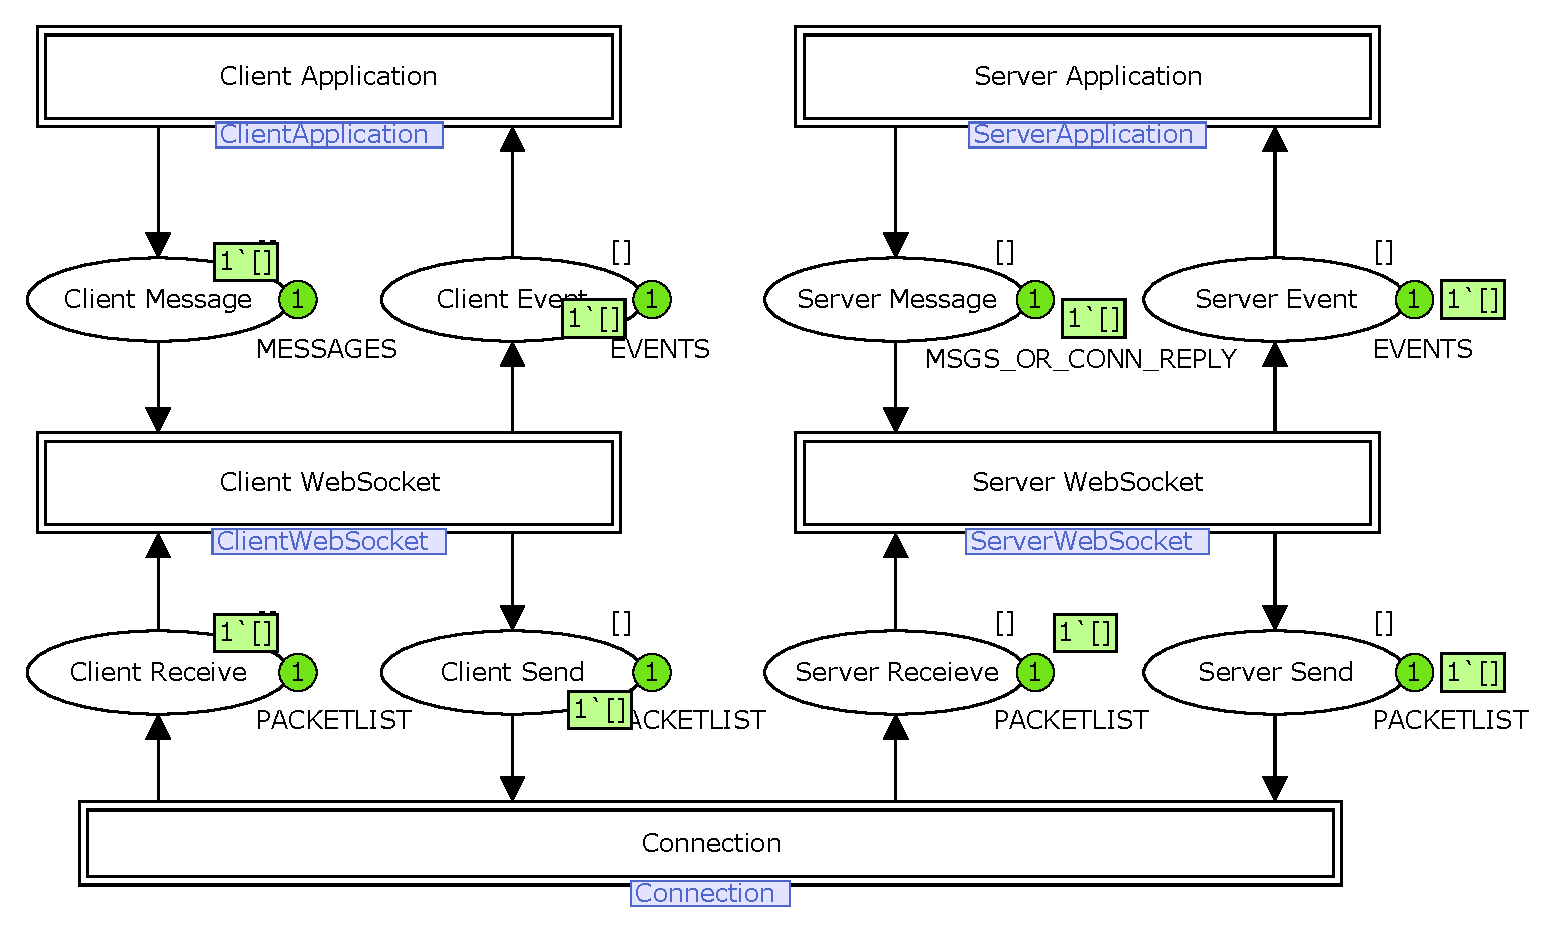
\includegraphics[scale=0.4]{figures/Overview.eps}
\caption{Overview of CPN model of the WebSocket protocol}
\label{fig:overview}
\end{figure}

Shown in Fig.~\ref{fig:overview} is the top-level overview of the WebSocket
protocol as a CPN model. 

Resembles part of OSI model (ref), where top level is levels 6 and 7, middle
level is level 5, and bottom level is levels 4 through 1. Two-way communication
between levels.

Circles represent places. They can contain tokens of a specified colour, and
can have markings to define initial tokens.

Double-bordered represent subpages. These are separate models that have
input and output places that connect to the places on their parent page. We will
examine the first subpage next.

\subsection{Client Application}

\begin{figure}
\centering
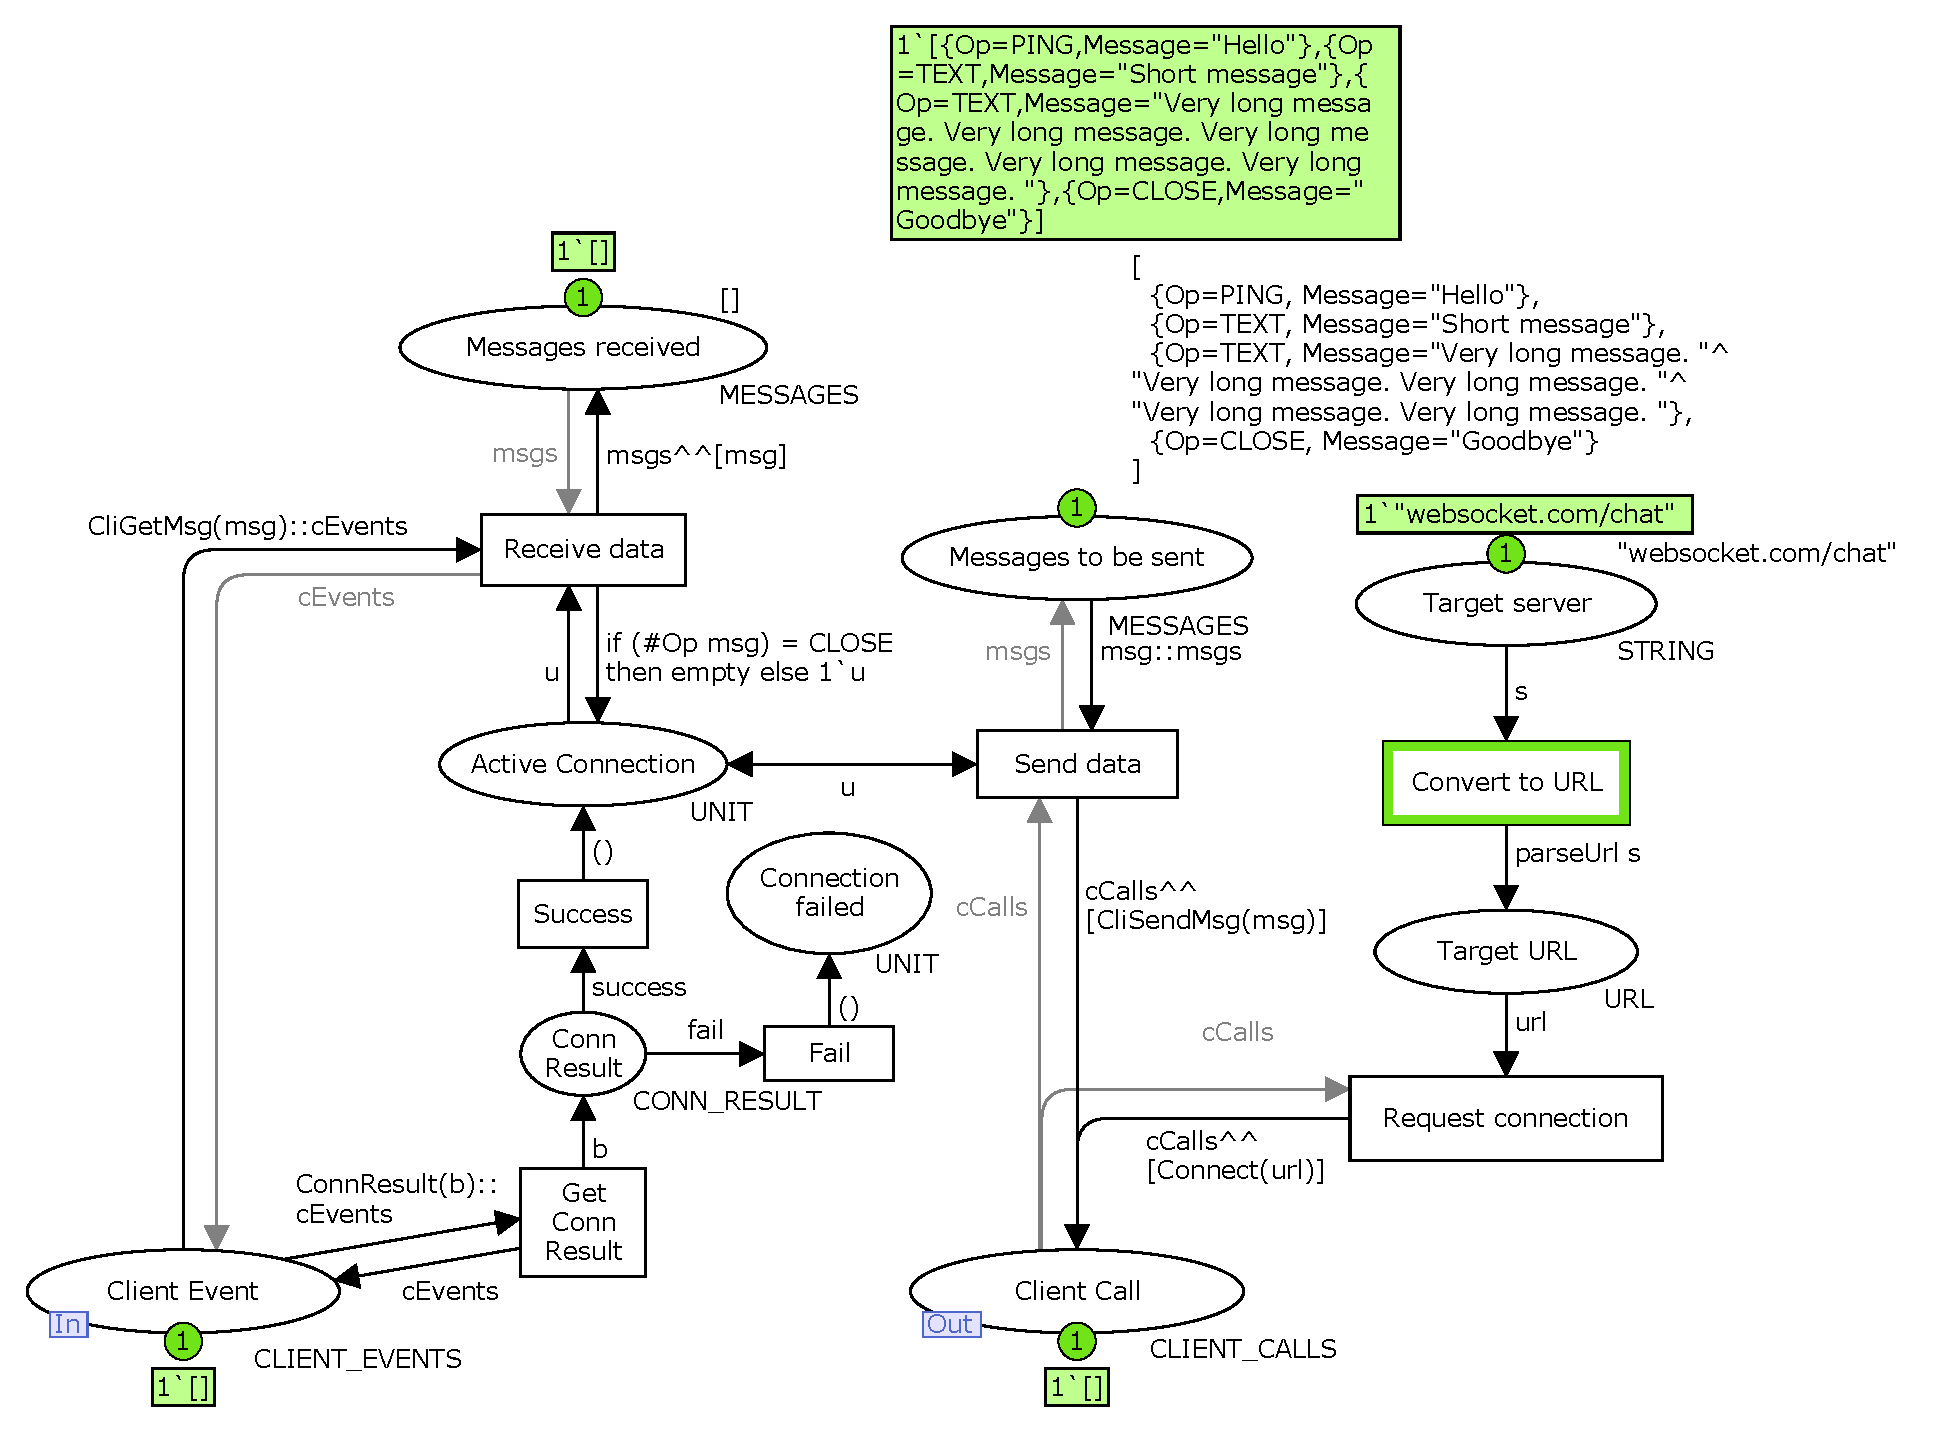
\includegraphics[scale=0.4]{figures/ClientApplication.eps}
\caption{The Client Application}
\label{fig:client_app}
\end{figure}

Laid out from top to bottom to loosely show sequence. 

Bottom places represent interface to WebSocket library. To simplify the overview
model and facilitate easier later expansion, we have only two places that act as
input and output, tagged In and Out. These are connected to the
respective places on the Overview, which are also connected to corresponding places in the
WebSocket Library.

Connect to server
Wait for result
Send and receive data

Here we see an enabled transition at the top. If we were to fire this
transition, it would produce a MESSAGE token in the Send Client Message place.

To the left we see a two-way arc between a place and a transition. This is a
technique used to simulate ordered processing of tokens; queues. We use
lists to do this. To describe a list in SML, we write [] for an empty list and
head::tail for a non-empty list, where head is the first element in the list,
and tail is all the following elements.

So, instead of using the actual color we want in the place, we use a list of
this color. When we want to take an element from the front of the queue,
we use the :: operator to bind the head and tail of the list to variables, and
put only the tail back to the source place. When we want to append an element
to a queue, we concatenate the queue using the \verb|^^| operator with a new
list containing only the new element. To improve readability of the model, these queue operations have
one arc slightly dimmed, to emphasise the flow direction of data.


\subsection{Client WebSocket Library}

\begin{figure}
\centering
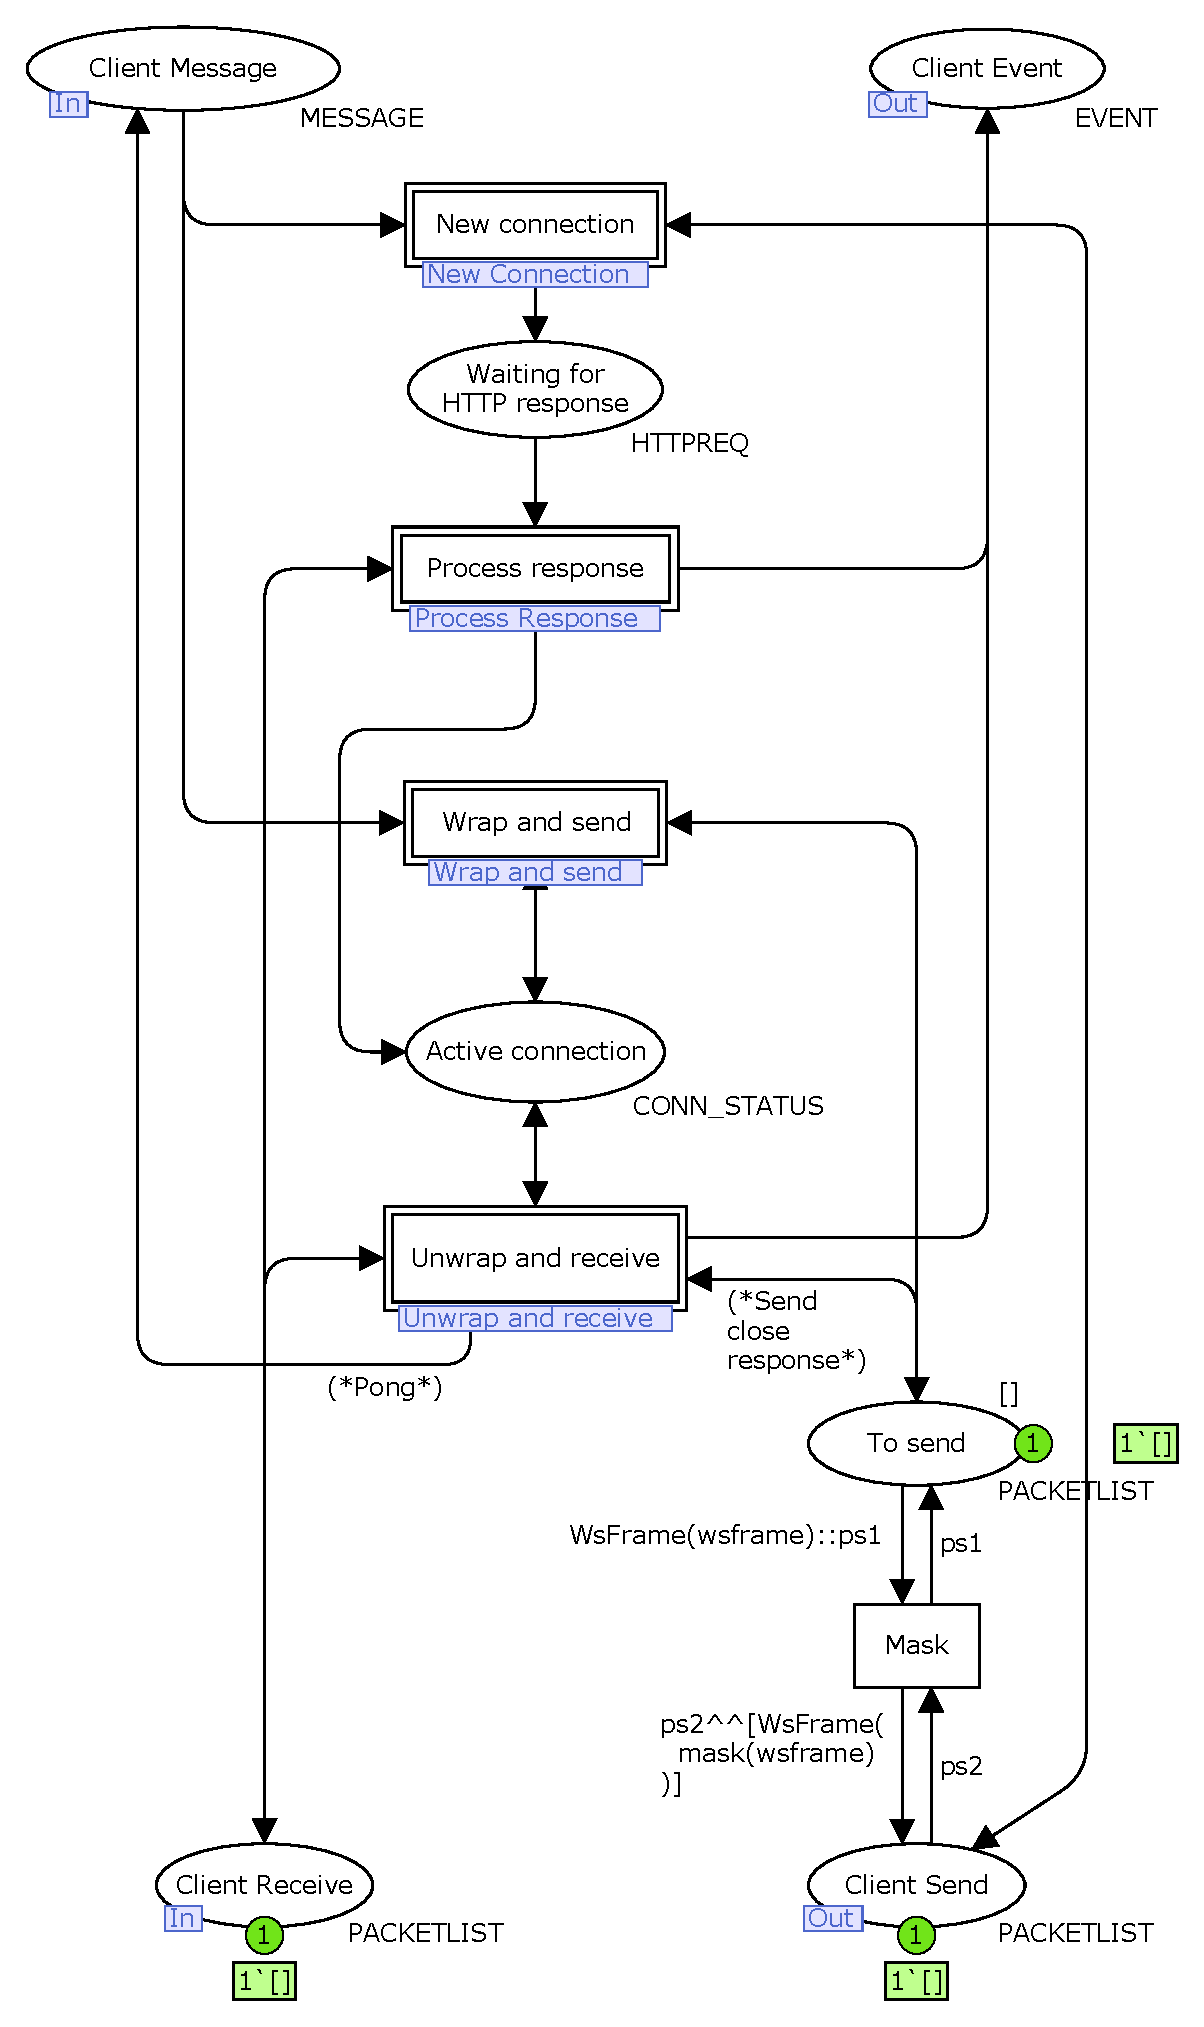
\includegraphics[scale=0.4]{figures/ClientWebSocket.eps}
\caption{The Client WebSocket Library}
\label{fig:client_wslib}
\end{figure}

This page consists mostly of subpages. The only processing being done here is
masking of all websocket frames.

\subsubsection{New connection}



\chapter{State Space Analysis of the WebSocket Protocol}
\label{chap:statespace}

One of the advantages of Coloured Petri Nets is the ability to conduct state
space analysis, which can be used to obtain information about the
behavioural properties of a CPN model, and which can be used to locate errors
and increase confidence in the correctness of the CPN model.

\section{State Spaces}
A state space is a directed graph where each node represents a reachable marking
(a state) and each arc represents an occurring binding element (a transition
firing with values bound to the variables of the transition). CPN Tools
by default generates the state space in breadth-first order. 

TODO: Figur av SS initiell modell, med forklaring

Once generated, the state space can be visualised directly in CPN Tools.
Starting with the node for the initial state, one can pick a node and show all
nodes that are reachable from it, and in this way explore the state space
manually. This can be very tedious and unmanageable for complex state spaces,
though, and instead it is usually better to use queries to automate the analysis
based on state spaces.

	\subsection{Strongly Connected Component graph}
	In graph theory, a strongly connected component (SCC) of a graph is a maximal
	subgraph where all nodes are reachable from each other. An SCC graph has a node
	for each SCC of the graph, connected by arcs determined by the arcs in the
	underlying graph between nodes that belong to different SCCs. An
	SCC graph is acyclic, and an SCC is said to be trivial if it consists of only
	one node from the underlying graph.
	
	By calculating the SCC graph of the state space, some of the further
	analysis becomes simpler and faster, such as determining reachability,
	cyclic behaviour, and checking so-called home and liveness properties. 

	\subsection{Application of State Spaces}
		The biggest drawback of state space analysis is the size a state spaces may
		become very large. The number of nodes and arcs often grows exponentially
		with the size of the model configuration.
		This is also known as the state explosion problem.
		
		\figDbl{ss/ClientApplicationNoMessagesCropped.eps}{Client}
		{ss/ServerApplicationNoMessagesCropped.eps}{Server}{Configuration:
		No messages}{ss_no_messages}
	
		This can be remedied by picking smaller configurations that encapsulate
		different parts of the system. This was necessary with the WebSocket Protocol
		model, as the complete state space took too long to generate with our
		original configuration (see \figref{client_app} and \figref{server_app}).
		We started by removing all messages to be sent (shown in
		\figref{ss_no_messages}).
		This means the only thing that should happen during simulation is the opening
		handshake. This configuration is used to explain the State Space Report in
		the next section.
		After this, we gradually added different types of messages to the client
		and/or server applications. These configurations will be discussed at the end
		of the chapter.
		
		Another aspect that must be considered prior to state space analysis is
		situations where an unlimited number of tokens can be generated, thus making
		the state space infinite. This can be remedied by modifying the model to
		limit the number of simultaneous tokens in the offending place.
		
		Additionally, a model that incorporates random values is not always suited
		for computing a state space. The generated state space depends on the random
		values chosen, so the state space generator needs to be able to
		deterministically bind values to arc expression variables.
				
		For small colour sets (generally defined as discrete sets usually with less
		than 100 possible values), binding of random values in arc expressions can
		occur in two ways: 
		\begin{enumerate}
		\item By calling ran() on the colourset. The ran() function picks a value
		ranging over the colour set, but since is non-deterministic, it isn't
		suited for state space generation.
		\item By using a free variable ranging over a colour set in the arc expression.
		A free variable is a variable that does not get assigned a value in an expression. It will 
		bind to a value picked at random from the colour set during simulation just
		like the ran() function, but also lets the state space generator pick each of 
		the possible bindings from the values available in the colourset, and thus
		generate all possible successive states. 
		\end{enumerate}
		
		For arc expressions that use type 1, it is usually possible to change or
		adapt it into type 2.
		
		Colour sets that use values from a large or unbounded range, or from continuous
		ranges like floating point numbers, are considered large colour sets, and using
		random values from such colour sets can make it impossible (or impractical)
		to generate a complete state space. It can be worked around by
		instead using small colour sets as described above. The CPN Tools manual has
		examples on how to do this.
		
		If these issues are not taken into account, a complete state space can not be
		achieved, since it's impossible for the state space genrator to make sure all
		possible values have been considered, and occurrence sequences might diverge
		if the same occurrence can happen in different orders but with different
		random values.
		
		For the WebSocket Protocol model, this was a problem for the masking
		key in WebSocket frames, which is supposed to be a random 4-byte string,
		giving $2^{32}$ or almost 4.3 billion possible values.
		To generate state spaces for this model, the randomisation function used was
		simply changed to always return four zeros. This is a reasonable abstraction
		since the specific value of the masking key does not affect the operation of
		the protocol. The result is shown in \lstref{fixed_masking_key}, with the old
		code commented out.
		
		\begin{lstlisting}[label=lst:fixed_masking_key,gobble=2,caption=Fixed masking
		key] 
		fun	randMask() = Mask([ 
			0,0,0,0
			(* BYTE.ran(), BYTE.ran(), BYTE.ran(), BYTE.ran() *)
		]);
		\end{lstlisting}
	
	\subsection{Visualisation}
	\fig[0.4]{ss/vis_NoMessages.eps}{No messages}{ss_vis_nomessage}
	CPN Tools can visualise a state space once it has been calculated.
	\figref{ss_vis_nomessage} shows the state space for the no messages
	configuration. Rounded squares represent markings, and arcs represent
	transition occurences. Clicking on the small triangle in the node will display
	a node descriptor which shows the marking that is associated with the node.
	Similarly, clicking on a state space arc will display an arc descriptor which
	describes the binding element associated with the arc. 

\section{State Space Report}
Once a partial or complete state space has been generated, CPN Tools lets the
user save a state space report as a textual document. The report is organised
into parts that each describe different behavioural properties of the state
space.

To explain each section of the state space report, a simple report for the
WebSocket protocol has been generated, in a configuration where no messages are
set to be sent. Thus, the only thing that will happen is that a connection will
be established. Later in the chapter we will consider more elaborate
configurations of the WebSocket protocol.
	
	\subsection{Statistics}
	The first section of the report describes general statistics about the state
	space.
	\begin{lstlisting}
  State Space
     Nodes:  17
     Arcs:   16
     Secs:   0
     Status: Full

  Scc Graph
     Nodes:  17
     Arcs:   16
     Secs:   0

	\end{lstlisting}
	This state space has 17 possible markings, with 16 enabled transition
	occurrences connecting them. There is one more node than there are arcs, which
	means this graph is a tree.
	
	The |Secs| field shows that it took less than one second to calculate this
	state space, while the |Status| field tells whether the report is generated
	from a partial or full state space. In this case the state space is fully
	generated.
	
	We also see that the SCC Graph has the same number of nodes and arcs, meaning
	that there are no cycles in the state space (although this was already known
	from the fact that it is a tree).
	
	\subsection{Boundedness Properties}
	The second section describes the minimum and maximum number of tokens for
	each place in the model, as well as the actual tokens these places can have.
	The text has been reformatted and truncated (indicated by [\ldots]) for
	readability.
	\begin{lstlisting}[language={}]
    Best Integer Bounds
                             Upper      Lower
     ClientApplication
          Active_Connection   1          0
          Conn_Result         1          0
          Connection_failed   0          0
          Messages_received   1          1
          Messages_to_be_sent 0          0
     [...]
	\end{lstlisting}
	
	Many places show a lower and upper bound of 1. This shows a weakness
	in the approach of using lists to facilitate ordered processing of tokens: We
	cannot see the actual number of tokens that are in each place, because
	technically there is just a list there. However, it quickly lets us know if
	something is wrong as well, since any values other than 0 or 1 here indicate a
	problem. 
	
	In fact, an error in the model was discovered this way, in the Unwrap and
	Receive module, where the pong reply was creating a new list instead of
	appending to the old one in outgoing messages. This caused the Client Outgoing
	Messages place to have 2 tokens at once. \figref{pong_fix} shows the location
	of the error before and after fixing it.
	\figDbl[0.35]{SSA_UnwrapAndReceive_Pong_before.eps}{Before}{SSA_UnwrapAndReceive_Pong_after.eps}{After}{Fixing
	Pong reply}{pong_fix}
	
	\begin{lstlisting}[language={},tabsize=4]
  Best Upper Multi-set Bounds
     ClientApplication
          Active_Connection		1`()
          Conn_Result			1`success
          Connection_failed		empty
          Messages_received		1`[]
          Messages_to_be_sent	empty
     [...]
     ClientWebSocket
          Connection_status		1`CONN_OPEN
     [...]
     ServerWebSocket
          Connection_Status		1`CONN_OPEN
     [...]

  Best Lower Multi-set Bounds
     ClientApplication
          Active_Connection		empty
          Conn_Result			empty
          Connection_failed		empty
          Messages_received		1`[]
          Messages_to_be_sent	empty
     [...]
     ClientWebSocket
          Connection_status		empty
     [...]
     ServerWebSocket
          Connection_Status		empty
     [...]
	\end{lstlisting}
	
	Apart from that, we see that both the client and the server has an open
	connection at some point, as the |Connection_status| place in the
	|ClientWebSocket| and |ServerWebSocket| modules have both had a |CONN_OPEN|
	token.
	
	\subsection{Home Properties}
	This section shows all home markings. A home marking is a marking that can
	always be reached no matter where we are in the state space. 
	\begin{lstlisting}[language={}]
  Home Markings
     [17]
	\end{lstlisting}
	We see that there is one such marking defined by node 17. From earlier we know
	that the state space is a tree, and if this node is always reachable it must be a leaf
	and all the other nodes must be in a chain. This agrees with the visualisation
	shown earlier, that there is only one possible sequence of transition
	occurrences to establish a connection. We can then confidently say that the
	model works correctly with this configuration. 
	
	\subsection{Liveness Properties}
	This section describes liveliness of the state space. Some of the transitions
	have been omitted for readability.
	
	\begin{lstlisting}[language={}]
  Dead Markings
     [17]

  Dead Transition Instances
     ClientApplication'Fail 1
     ClientApplication'Receive_data 1
     ClientApplication'Send_data 1
     ClientWebSocket'Filter_messages 1
     [...]

  Live Transition Instances
     None
	\end{lstlisting}
	
	A dead marking is a marking from where no other markings can be reached.
	 In other words, there are no transitions
	for which there are enabled bindings, and the system is effectivley stopped.
	For our example, we have a single dead marking, and it is the same as our home
	marking, confirming that this is a leaf node in the tree.
	
	We also get a listing of dead transition instances, which are transitions that
	never have any enabled bindings in a reachable marking and are thus never
	fired. This can be useful to detect problems with a model, but in this example
	it is expected for many of the transitions, since we are not sending any kind
	of messages in the configuration considered.
	
	Last, there are live transition instances. A transition is live if we from any
	reachable marking can find an occurrence sequence containing the transition.
	Our example has no such transition, which follows trivially from the fact that
	there is a dead marking.

	The state space report also contains fairness properties, but this does
	not apply to our model since it contains no cycles. We will not go into detail
	about this, and instead refer to \cite{cpn_book} chapter 7 for more
	information.
	
\subsection{Larger Configurations} 

	\subsubsection{One short message}
	The next step is to gradually increase the number of messages to be passed
	between the endpoints. We start by configuring the client to send a single
	message: |{Op=TEXT, Message="Short message"}|. 
	
	Here is part of the generated report:
	
	\begin{lstlisting}[language={}]
 Statistics
------------------------------------------------------------------------
  State Space
     Nodes:  29
     Arcs:   28
     Secs:   0
     Status: Full

  Home Markings
     [29]

  Dead Markings
     [29]

  Live Transition Instances
     None

     No infinite occurrence sequences.
	\end{lstlisting}
	
	The number of markings has not increased by much, and the other properties are
	largely the same, except there are fewer dead transition instances..
	The visualisation (\figref{ss_vis_1message}) shows there is still only one
	chain of occurrences.
	\fig[0.4]{ss/vis_1Message.eps}{One message}{ss_vis_1message}
	
	\subsubsection{One ping, then one message}
	When we add another message to be sent (a ping, which will also result in a
	pong being sent back), we see that the number of nodes has increased by an
	order of magnitude:
	
	\begin{lstlisting}[language={}]
  State Space
     Nodes:  475
     Arcs:   1140
     Secs:   1
     Status: Full
     
  Home Markings
     [475]

  Dead Markings
     [475]
	\end{lstlisting}

	CPN Tools supports exporting state spaces to a format supported by Graphviz, an
	open source application for visualising graphs. We have used Graphviz to
	visualise this state space, shown in \figref{ss_vis_1ping1message}. This
	clearly demonstrates the effect of the state space explosion problem.
	
	\fig[0.145]{ss/vis_1ping1message.eps}{One ping, one
	message}{ss_vis_1ping1message}

	\subsubsection{One message, then one ping}
	By reversing the order of the two messages, the state space gets slightly
	larger, due to the fact that WebSocket could send the ping frame first, since
	it is a control frame.
	
	\begin{lstlisting}[language={}]
  State Space
     Nodes:  513
     Arcs:   1141
     Secs:   1
     Status: Full
     
  Home Markings
     None

  Dead Markings
     [512,513]
	\end{lstlisting}
	Note that we now no longer have any home marking, and instead have two dead
	markings, representing the two possible orderings of the two messages.
	
	\subsubsection{One long message}
	We now set a message that is large enough to require fragmenting. 
	|{Op=TEXT,Message="Very long message. Very long message. Very long message. Very long message. Very long message. "}|
	
	\begin{lstlisting}[language={}]
  State Space
     Nodes:  813
     Arcs:   2331
     Secs:   2
     Status: Full
     
   Home Markings
     [813]

  Dead Markings
     [813]
	\end{lstlisting}
	We see this has more states than sending two simple messages. We can also use
	the Best Upper Multi-set Bounds section to find the largest collection of
	fragments.
	\begin{lstlisting}[language={},gobble=1]
	1`[WsFrame({Fin=clear,Rsv1=clear,Rsv2=clear,Rsv3=clear,Opcode=1,Masked=set,Payload_length=20,Masking_key=Mask([0,0,0,0]),Payload="Very long message. V"}),
	WsFrame({Fin=clear,Rsv1=clear,Rsv2=clear,Rsv3=clear,Opcode=0,Masked=set,Payload_length=20,Masking_key=Mask([0,0,0,0]),Payload="ery long message. Ve"}),
	WsFrame({Fin=clear,Rsv1=clear,Rsv2=clear,Rsv3=clear,Opcode=0,Masked=set,Payload_length=20,Masking_key=Mask([0,0,0,0]),Payload="ry long message. Ver"}),
	WsFrame({Fin=clear,Rsv1=clear,Rsv2=clear,Rsv3=clear,Opcode=0,Masked=set,Payload_length=20,Masking_key=Mask([0,0,0,0]),Payload="y long message. Very"}),
	WsFrame({Fin=set,Rsv1=clear,Rsv2=clear,Rsv3=clear,Opcode=0,Masked=set,Payload_length=15,Masking_key=Mask([0,0,0,0]),Payload=" long message. "})]
	\end{lstlisting}
	We are also able to inspect every other possible combination, and can thus
	confirm that messages are being split correctly.

	\subsubsection{Ping, text, close}
	With three messages, state space calculation becomes noticeably time-consuming.
	
	\begin{lstlisting}[language={}]
  State Space
     Nodes:  6129
     Arcs:   19625
     Secs:   14
     Status: Full
     
       Dead Markings
     6 [6129,6112,6029,5960,5632,...]
	\end{lstlisting}
	
	Here we have six dead markings. In half the cases, the close is sent before
	the text. For each of those halves, the three cases consist of the pong frame
	either successfully arriving at the client, not being received by the client due
	to the connection being closed, or not being sent from the server for the same
	reason. This was verified by manual inspection in CPN Tools.

	\subsubsection{Even larger configurations}
	We tried adding one more message to the server application, but after running for
	5 hours the state space calculation had still not been able to compute a
	complete state space. Fortunately, it is still possible to create a report for
	the partial graph. 
	\begin{lstlisting}[language={}]
  State Space
     Nodes:  165748
     Arcs:   707380
     Secs:   18000
     Status: Partial
	\end{lstlisting}
	The report also showed that it had not found any cycles, which reinforces the
	claim that the model works as it should.

\chapter{Technology and foundations}
\label{chap:technology}

One of the first decisions that had to be made for this thesis was whether to
base the work on an existing platform or to create a new one from
scratch. In this chapter we will describe the reasoning behind our choices, and
give an overview of the technologies that have been used.

\section{(decision)}\com{Finne på tittel}
	A simple but easy way of manipulating a CPN model is by representing it as a
	tree. Simple tree editors are a feature of most GUI software platforms. Even
	so, we realised early that writing everything from scratch would probably take
	much longer than adapting an existing platform.

	There are of course many complete implementations of Petri Net tools in
	different languages and toolkits, but few of them are open source, or written with
	extensibility in mind. If we were to base our work on an existing platform, it
	would have to be open and extendable. 
	
	To narrow our search, we limited our options to solutions in
	languages we had experience with: Java, c++/Qt and Ruby. Java is a popular
	language, and we already have Access/CPN, a part of the CPN Tools project,
	which can parse .cpn files into Java objects. 
	
	By searching the web, we discovered the ePNK framework, an extendable framework
	for working with Petri Nets in a graphical manner, and lets you specify your
	own Petri Net type. It is built on the Eclipse Modeling Framework (EMF) (which
	Access/CPN is also built on).
	
	We also needed a way to represent pragmatics. It was suggested to try an
	ontology-based approach, and we decided on SADL, another Eclipse plugin that
	lets us easily define and work with ontologies.
	
	\fig{AppOverviewDiagram.pdf}{Application Overview Diagram}{app_overview}
	
	\figref{app_overview} shows the different elements that make up the application.
	The elements with bold frames are the ones newly created for this thesis, while
	the rest below are the existing solutions used and built upon. These will be
	described in the following sections, from the bottom up.

\section{Eclipse IDE}
Eclipse IDE is an open source, cross-platform, polyglot development environment.
Its plugin framework makes it greatly extendable and customisable, and especially makes it
easy for developers to quickly create anything from small custom macros, to
advanced editors, to whole applications. The Eclipse IDE is open source, and
part of the Eclipse Project, a community for incubating and developing open
source projects.

\fig{EclipsePlatformDiagram.pdf}{The Eclipse RCP}{eclipse_rcp}

The Eclipse IDE is built on the Eclipse Rich Client Platform (RCP),
\figref{eclipse_rcp}. At the bottom of this we have the Platform Runtime, based
on the OSGi framework, which provides the plugin architecture. The other
plugins shown in the diagram together form a basic generic IDE.

The principal Eclipse distribution is the Eclipse Java IDE, which is one of the
most popular tools for developing all kinds of Java applications, from small
desktop applications, to mobile apps for Android, to web applications, to
enterprise-scale solutions. 

Plugins are the building blocks of Eclipse, and there exists a wide range of
plugins that add tools, functionality and services. For example, this thesis
was written in \LaTeX{} using the Texlipse plugin, and managed with the Git
version control system through the EGit plugin. 

Publishing a custom plugin is simple. By packaging it and serving it on a
regular web server, anyone can add the web server url to the update manager in
Eclipse, and it will let you download and install it directly, as well as
enabling update notifications.

It is possible to package Eclipse with sets of
plugins to form custom editions of Eclipse that are tailored for specific
environments and programming languages. Aptana Studio is one example, aimed at
Ruby on Rails and PHP development.


\section{Eclipse Modeling Framework}
EMF is a framework for Model Driven Development (MDD) in Java. It is an Eclipse
plugin that is part of the Eclipse Platform, and open source. By providing
modeling and code generation tools, it lets developers create model
specifications that can be converted to Java classes, along with a
set of adapter classes that enable viewing and command-based editing of the
model, and a basic editor. \com{prøve å utvide, men vanskelig å finne noe mer
fornuftig å skrive}

	\subsection{Graphical Modeling Framework}
	GMF builds on EMF to provide graphical viewing and editing of models. It uses
	metamodels created with EMF to generate implementations of views and editors
	that can create and edit the respective models. 

\section{ePNK: Petri Net framework}
ePNK is an Eclipse plugin both for working with standard Petri Net models, and a
platform for creating new tools for specialised Petri Net types, which is
exactly what we need for our annotated CPN. It uses EMF and GMF to work with the
Petri Net models and provide generic editors for custom Petri Net variants.

There are several reasons why ePNK is a good choice:
\begin{itemize}
	\item It saves models using the ISO/IEC 15909 \com{referanse?} standard file
	format PNML,
	\item It is currently actively developed,
	\item It is designed to be generic and easily extendable by creating new model
	types, and
	\item It includes both a tree editor and a graphical editor, provided through
	GMF.
\end{itemize}

ePNK includes definitions for the core PNML model type, as well as two
subtypes of Petri Nets. The first is P/T-Nets, or Place/Transition Nets, which
expand on the core model with a few key items: initial markings for places,
inscriptions on arcs, and constraining arcs to only go between a place and a
transition (this is not enforced in PNML, as there are Petri Net variants that
allow this). 

The other is High level Petri nets (HLPNG). This type adds several more labels,
all of which are Structured Labels. These are parsed and validated using a
syntax that is inspired from (but not the same as) CPNML from CPN Tools. It is
possible to write invalid data in these labels and still save the document, as
they will only be marked as invalid

Neither of these two conform exactly to the Coloured Petri Nets created by CPN
Tools. HLPNG comes close, but is missing a few things like ports and sockets
(RefPlaces can emulate this), and substitutin transitions. Also, the
structured labels are not compatible with CPNML syntax from CPN Tools, and for
our prototype, these structured labels are not necessary with regard to
annotations. It is possible that this might be useful in a future version,
where for example pragmatics are available depending on things like the
colorset of a place or the variables on an arc, but this would take too much
time to implement. \com{Bedre formulering av siste setning?}

Our decision was to develop our own Petri net type, which matches CPN Tools as
close as possible.

\section{Access/CPN: Java interface for CPN Tools}
CPN Tools has a sister project called Access/CPN. This is an
EMF-based tool to parse .cpn files and represent them as an
EMF-model. The .cpn files saved by CPN Tools are XML-based, which makes them
easy to parse, but having an existing solution for this is preferrable.

The model definition used by Access/CPN is very similar to that of ePNK.
\com{Diskutere mer i implementation?}

TODO: Vurdere å utvide med egen algoritme som konverterer direkte til ePNK?

\section{SADL: Ontologies}
Ontologies are a way to present information and meta-information so that it can
be understood by computers. Essentially, this is done by defining classes that
have properties, relations and constraints, and then association
information with these classes.

There is a lot of ongoing research on this subject, especially to create a
semantic web, that is extending web pages to provide meta-information about the
content they contain and enabling software to understand it and reason about it. 

SADL is an Eclipse plugin that defines an english-like syntax for defining
ontologies, and comes with a text editor that features syntax highlighting,
parsing and validation. This is useful as we can possibly reuse the editor in
our plugin for defining model-specific pragmatics.

It also has tools to parse and reason with these ontologies, which we will use
to filter and validate which pragmatics are available for different model
entities.

\section{Summary}
After picking these technologies, since all the componets have Eclipse in
common, it was an easy decision to develop our project as an Eclipse plugin.
This also let us centralise all our development in Eclipse.

\chapter{Analysis and Design}
\label{chap:analysis}

Lorem ipsum dolor sit amet, consectetur adipiscing elit. Sed elit purus, cursus eget pellentesque et, tristique id neque. Sed non quam ac sem malesuada aliquet vitae in massa. Donec a lectus enim, a porttitor velit. Sed rutrum risus non sem ultricies sit amet sollicitudin elit consequat. Quisque tincidunt vulputate lacus, id ornare nisi porta sit amet. Ut congue leo eget nisl semper lacinia. Etiam vitae tortor at diam rhoncus convallis. Vestibulum id metus ante.

\section{Analysis}

Donec sapien tellus, luctus vel molestie ut, pulvinar et tellus. Nunc cursus hendrerit egestas. Etiam pellentesque condimentum metus ut rhoncus. Maecenas eu leo velit, vitae lobortis augue. Pellentesque ullamcorper est ut felis ultricies eu pharetra neque pharetra. Praesent vitae sapien quis ligula hendrerit sagittis id ut sem. Praesent orci quam, molestie vestibulum eleifend id, laoreet tempus dolor. Duis in enim vitae ante mattis molestie vitae imperdiet justo. Sed lorem erat, mollis consequat molestie sit amet, lacinia vulputate lectus. Nunc risus metus, rutrum sit amet aliquet ut, faucibus quis urna. Vestibulum ac turpis ante. Aliquam mauris magna, volutpat malesuada bibendum sed, tempor a magna. Morbi erat enim, vestibulum at mattis eget, dictum at magna.

Morbi ullamcorper enim eu odio gravida et convallis augue feugiat. Ut ut suscipit lorem. Donec tristique facilisis velit, fermentum lobortis massa vestibulum nec. Mauris scelerisque dignissim scelerisque. Duis eu sem dui. Nulla et tortor non urna accumsan congue. Donec neque justo, vestibulum id dignissim venenatis, cursus eu orci. Phasellus vitae placerat mi. Cum sociis natoque penatibus et magnis dis parturient montes, nascetur ridiculus mus.

\section{Design}
Ut nibh massa, faucibus bibendum tempus adipiscing, pretium ac nunc. Cras id imperdiet urna. Suspendisse potenti. Vestibulum hendrerit laoreet arcu, eu congue velit mattis id. Proin aliquam elementum diam sed placerat. Nam mollis mauris id tortor iaculis scelerisque. Nam vel tortor et nunc condimentum dignissim. Fusce ut leo id eros consectetur pharetra at non velit. Vestibulum hendrerit purus quis libero euismod adipiscing. Integer bibendum fermentum viverra. Pellentesque fermentum sapien et eros dignissim pellentesque elementum felis ornare.

Cras scelerisque bibendum convallis. Maecenas laoreet imperdiet lacinia. Fusce ornare augue vitae tortor scelerisque ut rhoncus enim mollis. Quisque non justo mauris. Quisque dolor nulla, feugiat a fringilla sit amet, tempus in dui. Nulla facilisi. Fusce sodales diam quis risus ultricies posuere. Integer et semper mi. In hendrerit tortor a dolor faucibus posuere.

%\chapter{Implementation}
\label{chap:implementation}

Lorem ipsum dolor sit amet, consectetur adipiscing elit. Sed vulputate ornare sagittis. Nam rutrum condimentum dolor at bibendum. Quisque quis massa tellus. Sed luctus mauris sit amet metus lacinia eleifend. Mauris malesuada tellus eget dui convallis id porttitor diam porta. Sed mollis velit a quam condimentum euismod. Sed hendrerit neque et nulla suscipit ac eleifend arcu congue. Suspendisse nisi mi, accumsan non elementum nec, aliquam sed justo. Vivamus eu arcu lorem. Vestibulum a ante nibh, a dignissim lorem. Etiam laoreet ante a est blandit a pellentesque lorem laoreet. Phasellus id velit mauris, et lacinia purus. Sed sodales iaculis vulputate.


\section{Conversion from CPN Tools to ePNK}
Fusce pellentesque, mauris nec fermentum vehicula, ligula turpis dictum ante, ac gravida erat orci vitae libero. Sed ac tellus eros. Nulla facilisi. Suspendisse potenti. Nullam massa leo, viverra at imperdiet id, interdum a nibh. Integer convallis aliquet dapibus. Phasellus sed nisl erat. Curabitur at lacus ligula, non lobortis velit. Suspendisse potenti. Curabitur in velit in est cursus commodo.

Vestibulum in nisi eu risus euismod dapibus. Nam vel lorem ipsum, vel mollis mi. Morbi sed velit sit amet enim commodo fringilla. Nunc dui ante, sodales eget mollis a, commodo porta elit. Fusce urna est, aliquet a pellentesque sit amet, vehicula nec leo. Morbi in dui leo. Class aptent taciti sociosqu ad litora torquent per conubia nostra, per inceptos himenaeos. Ut purus magna, consequat vel semper eget, hendrerit ut massa. Maecenas pulvinar lacus a neque pulvinar congue. Ut malesuada commodo erat, non posuere massa fermentum ut. Proin suscipit sodales bibendum. Ut id dolor mauris, commodo eleifend neque. Etiam interdum interdum euismod. Ut lobortis malesuada pellentesque. Nullam venenatis volutpat ornare. Donec varius elit at elit adipiscing lobortis.

\subsection{Access/CPN}
Aliquam erat volutpat. Praesent ullamcorper commodo augue in faucibus. Sed et tortor non arcu aliquam pharetra. Sed odio massa, pharetra ut faucibus sed, rhoncus vel lectus. Morbi consequat purus at ipsum placerat vel dapibus justo dignissim. Etiam feugiat pulvinar tempus. Fusce vestibulum odio a leo porttitor at pulvinar velit egestas. Praesent at venenatis lectus. Donec gravida, lacus vitae tincidunt tincidunt, risus leo congue mi, vitae pharetra magna ipsum eget dui. Suspendisse suscipit mollis pellentesque. Nunc ac nulla sit amet diam tincidunt volutpat quis in eros. Integer diam odio, mollis ac porta eget, faucibus vel mi. Maecenas vitae mauris tellus. Aliquam vel fringilla arcu. Praesent ut magna massa, ut dignissim massa.

Aenean porttitor massa non quam euismod laoreet. Nam quis nulla sem. Donec hendrerit, orci a ultrices viverra, orci mi ultricies nibh, eu vestibulum nulla eros ac ligula. Donec velit nisi, rhoncus nec pharetra sit amet, pretium sit amet turpis. Nullam scelerisque elit eu nisi vulputate vel imperdiet odio luctus. Maecenas laoreet ante ac elit consequat ullamcorper. Nunc lorem tellus, hendrerit luctus pulvinar tempus, molestie nec mi. Nam sem sapien, aliquam imperdiet tincidunt eu, elementum eu ipsum. Curabitur sed risus at lacus tincidunt rutrum. Praesent id lorem mi. Pellentesque habitant morbi tristique senectus et netus et malesuada fames ac turpis egestas.

\chapter{Evaluation}
\label{chap:evaluation}

Lorem ipsum dolor sit amet, consectetur adipiscing elit. Maecenas faucibus libero at lorem accumsan at ullamcorper tellus facilisis. Nulla nec metus ligula. Vivamus varius est vitae nisl bibendum porttitor. Suspendisse arcu orci, rhoncus et accumsan non, hendrerit id urna. Aliquam dictum molestie quam, ac imperdiet dui hendrerit in. In posuere laoreet faucibus. Cras sit amet dui risus, gravida condimentum diam. Nullam turpis lacus, lobortis a egestas ac, ultrices et nisl.


\section{Requirements}
Curabitur consequat odio vel dui laoreet rutrum. Praesent pretium lorem a nibh tempus non elementum sem varius. Sed bibendum quam elementum diam vehicula at tempus ipsum cursus. Mauris dui tellus, luctus non tincidunt ac, placerat sit amet metus. Class aptent taciti sociosqu ad litora torquent per conubia nostra, per inceptos himenaeos. Aliquam nec sem ac purus condimentum facilisis. Pellentesque eu libero nec mi faucibus bibendum. Aliquam erat volutpat. Proin id dignissim nunc. Vivamus porttitor pharetra ipsum, in luctus tellus fermentum luctus. Mauris tristique, justo vel blandit venenatis, elit ante volutpat ligula, vitae lobortis nisl magna nec risus. Nullam ultricies porttitor leo non mattis. Pellentesque habitant morbi tristique senectus et netus et malesuada fames ac turpis egestas.

Phasellus imperdiet, dolor feugiat iaculis pharetra, orci nisi blandit mi, sed consectetur justo tellus suscipit eros. Donec non leo purus. Nulla feugiat lorem ut nunc blandit in rhoncus justo lobortis. Nulla facilisi. Vivamus urna mauris, volutpat vitae facilisis nec, aliquet vitae mi. Nullam in ante sem, nec malesuada est. Etiam pharetra eleifend sagittis. Vestibulum id enim nec eros rhoncus consequat id ut diam. Nulla cursus ultricies velit eu vehicula. Aenean luctus augue eget mauris tempor accumsan. Maecenas purus enim, mollis quis aliquam quis, placerat ac purus. Vestibulum quis lectus velit, sed ultrices ligula. Maecenas eget porttitor tortor. Pellentesque ut lorem ipsum.

\section{User Feedback}
Vivamus vitae mi quam, vitae fermentum elit. In blandit nulla quis metus vulputate ultricies. Integer malesuada sagittis interdum. Maecenas vestibulum tortor risus, id ultrices massa. Aenean pharetra velit vel enim euismod a sodales odio euismod. Curabitur nisi mi, feugiat vitae sollicitudin non, porta eget nisi. Nulla mollis, dui id bibendum molestie, augue ante gravida dolor, a laoreet sem est sollicitudin elit. Quisque ac purus leo.

Aenean eget urna eu sapien tincidunt lobortis. Duis id dolor quam, vel feugiat libero. Duis tempor, sem id feugiat consectetur, ante nibh convallis quam, hendrerit hendrerit dolor dui in velit. Proin sagittis ante in nisi tempor vel commodo augue bibendum. Proin eu quam id lectus tristique luctus. Donec a risus ut erat tristique posuere ut eu magna. Phasellus suscipit mi vel ipsum pretium elementum in blandit nisi.

\chapter{Conclusion}
\label{chap:conclusion}

With \thename{}, we have constructed a fully functional proof of concept that
demonstrates the advantages and disadvantages of using ontologies to manage code
generation pragmatics and applying them to a CPN model. As shown in Chapter
\ref{chap:analysis}, this prototype meets all of the requirements in Section
\ref{sec:requirements}. Through our evaluation by using it to annotate CPN
models of different sizes, we have shown that using ontologies gives a highly
expressive means to defining pragmatics as well as providing automatic
validation of the annotated model. However ontology reasoning using CWA yields
decreasing performance as model size increases, to a point that makes our
prototype unusable for the WebSocket CPN model. Still, we believe our approach
has potential, and warrants further optimisation and research.

\section{Future work}

Continue the work of Simonsen, defining more general and domain-specific
pragmatics. Also, assert required configuration arguments.

Finding or developing ontology reasoner tailored for CWA.

A specialised tool for creating model specific pragmatics would have been ideal.
Such a tool would give simple mechanics using GUI controls for specifying which
model elements a pragmatic can be attached to, and which parameters it has. The
Plugin Manifest editor is a good example of what we have in mind. However, this
could not be included for this thesis due to time constraints.

Implement structured labels for the CPN Type. Could enable placement of
pragmatics inside expressions.

When importing, let user choose between CPN and Pragma CPN. Alternatively,
mechanic for upgrading the Type.

Accurately model sub-modules, ports and sockets. This enables more advanced
pragmatics; for instance the Principal pragmatic could be specified to only be
available for substitution transitions on top-level modules.

\section{Acknowledgments}

Thank supervisor Lars Michael Kristensen

Kent Inge Fagerland Simonsen 

Michael Westergaard for help with Access/CPN

Ekkart Kindler for extensive help with ePNK

\appendix
\bibliographystyle{alpha}\bibliography{literature,rfc}
\listoffigures
\lstlistoflistings


\end{document}
